\section{Esempio Pratico in Python}
Per illustrare questi concetti, consideriamo un esempio pratico in Python. Abbiamo misurato le altezze di 100 persone (in cm) e calcoleremo la media, la deviazione standard e la deviazione standard della media di queste misure. Successivamente, creeremo un istogramma delle altezze e lo sovrapporremo con la curva gaussiana corrispondente.

\begin{lstlisting}[language=Python, caption={Script Python per calcolare e visualizzare le altezze}]
import numpy as np
import matplotlib.pyplot as plt
from scipy.stats import norm

# Altezze di 100 persone (in cm)
heights = [170, 165, 180, 175, 160, 155, 178, 172, 168, 169, 
           174, 167, 166, 171, 173, 177, 182, 181, 176, 179, 
           164, 163, 162, 161, 159, 158, 157, 156, 154, 153, 
           152, 151, 150, 149, 148, 147, 146, 145, 144, 143,
           150, 155, 160, 165, 170, 175, 180, 185, 190, 195,
           172, 177, 182, 187, 192, 197, 162, 167, 172, 177,
           180, 175, 170, 165, 160, 155, 150, 145, 140, 135,
           142, 147, 152, 157, 162, 167, 172, 177, 182, 187,
           165, 170, 175, 180, 185, 190, 195, 200, 205, 210]

# Stima di media, deviazione standard e deviazione standard della media
mu = np.mean(heights)
sigma = np.std(heights, ddof=1)
sigma_x_mean = sigma / np.sqrt(len(heights))

# Arrotonda la deviazione standard della media e la media alle unità
sigma_x_mean_rounded = round(sigma_x_mean)
mu_rounded = round(mu)

print(f"Media delle altezze: {mu_rounded} cm")
print(f"Deviazione standard delle altezze: {sigma:.2f} cm")
print(f"Deviazione standard della media: {sigma_x_mean_rounded} cm")

# Creazione dell'istogramma
count, bins, ignored = plt.hist(heights, bins=6, density=True, alpha=0.6, color='g', edgecolor='black')

# Sovrapposizione della curva gaussiana
xmin, xmax = plt.xlim()
x = np.linspace(xmin, xmax, 100)
p = norm.pdf(x, mu, sigma)
plt.plot(x, p, 'k', linewidth=2)
title = "Istogramma delle Altezze e Curva Gaussiana"
plt.title(title)

# Visualizzazione di media e deviazione standard
plt.axvline(mu, color='r', linestyle='dashed', linewidth=1)
plt.text(mu + mu/10, max(p), f'Media: {mu_rounded} cm', color='r')
plt.axvline(mu + sigma, color='b', linestyle='dashed', linewidth=1)
plt.axvline(mu - sigma, color='b', linestyle='dashed', linewidth=1)
plt.text(mu + sigma + mu/10, max(p)/2, f'Sigma: {sigma:.2f} cm', color='b')
plt.text(mu - sigma - mu/10, max(p)/2, f'Sigma: {sigma:.2f} cm', color='b')

# Impostazione dei valori sui bins come etichette sull'asse x
bin_labels = [f"{int(bins[i])}" for i in range(len(bins))]
plt.xticks(bins, labels=bin_labels, rotation=45)

# Migliora la disposizione dei sottotitoli e delle etichette
plt.tight_layout()

plt.savefig('istogramma.png')
#se vuoi scaricare il file da google colab decommenta le righe:
#from google.colab import files
#files.download('istogramma.png')
plt.show()

# Risultato finale, arrotondato a due cifre significative
print(f"Altezza = ({mu_rounded} +- {sigma_x_mean_rounded}) cm")
\end{lstlisting}

\subsection{Significato delle Variabili, Moduli, Funzioni e Parametri}
Spieghiamo brevemente il significato delle variabili, dei moduli usati, delle funzioni e dei parametri:

\begin{itemize}
    \item \texttt{numpy} (\texttt{np}): Una libreria per il calcolo numerico in Python. Utilizzata per calcolare la media (\texttt{np.mean}) e la deviazione standard (\texttt{np.std}) delle altezze.
    \item \texttt{matplotlib.pyplot} (\texttt{plt}): Una libreria per la creazione di grafici. Utilizzata per creare l'istogramma (\texttt{plt.hist}) e sovrapporre la curva gaussiana (\texttt{plt.plot}).
    \item \texttt{scipy.stats.norm}: Fornisce la funzione di densità di probabilità per una distribuzione normale. Utilizzata per calcolare la curva gaussiana da sovrapporre all'istogramma.
    \item \texttt{plt.hist()}: Funzione per creare un istogramma. Il parametro \texttt{bins} definisce il numero di intervalli.
    \item \texttt{plt.plot()}: Funzione per tracciare una linea su un grafico. Utilizzata per disegnare la curva gaussiana.
    \item \texttt{np.linspace()}: Funzione per generare una sequenza di numeri spaziati uniformemente. Utilizzata per generare i valori x della curva gaussiana.
\end{itemize}

Ecco l'output:
\begin{verbatim}
Media delle altezze: 167.83333333333334 cm
Deviazione standard delle altezze: 15.80 cm
Deviazione standard della media: 1.67 cm
Altezza = (168 +- 2) cm
\end{verbatim}
Nel grafico \ref{fig:istogramma} vediamo sovrapposto l'istogramma costruito e la curva che lo approssima. L'istogramma ha in ascisse (asse X) gli intervalli di altezza e in ordinate (asse Y) un valore tale che l'area del bin sia uguale alla frazione di persone che hanno un'altezza compresa tra i suoi estremi. Ad esempio, se guardiamo l'intervallo tra 160 e 172, l'altezza è 0,025 perché $\left(172-160 \right)\times 0,025 =0,3$ ossia, il 30\% delle persone aveva un'altezza compresa tra 160 e 172 centimetri. Ancora un commento su media e deviazione standard. Notare che la curva è centrata attorno alla media (il valore $\SI{167,3}{\centi\meter}$) evidenziata dalla linea rossa tratteggiata. Notare anche le due linee blu. La distanza tra la linea verde e quella blu è proprio uguale alla deviazione standard (pari a $\SI{15,80}{\centi\meter}$ e indicata sul grafico come \textit{Sigma}), infatti $\SI{167,83}{\centi\meter} + \SI{15,80}{\centi\meter} = \SI{183,63}{\centi\meter}$ che è proprio dove si trova la linea verde. Notiamo infine che il 68\% delle misure capitano tra i valori $\SI{167,83}{\centi\meter} -\SI{15,80}{\centi\meter}$ e $\SI{167,83}{\centi\meter} +\SI{15,80}{\centi\meter}$, ossia tra $\SI{152,03}{\centi\meter}$ e $\SI{183,63}{\centi\meter}$. Questo è sempre vero. Quando abbiamo una grandezza che si distribuisce come la curva a campana (la gaussiana scoperta dallo scienziato Gauss) l'area sotto la curva, quella compresa tra le due linee blu, è sempre 0,68 ossia il 68\% delle misure che la approssimano, dovrebbero capitare tra $\overline{x} -\sigma$ e $\overline{x} + \sigma$.

\begin{figure}[h!]
    \centering
    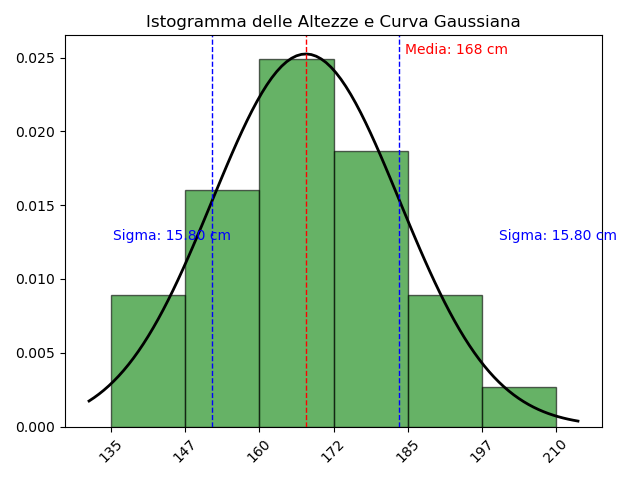
\includegraphics[width=0.8\textwidth]{istogramma.png}
    \caption{Istogramma delle Altezze con Sovrapposta la Curva Gaussiana}
    \label{fig:istogramma}
\end{figure}


